\chapter{PROCEDURE} \label{ch:procedure}
Each team is provided with 4 column cards such as TO DO, DOING, TEST, DONE and
9 task cards (actually colorful sticky notes). Team members selected task according to
their choice. The first step is to do independent works such as ”Data Collection”. I was
assigned task 4 and 6 which were to collect data of ages and favorite food of all team
members.
\begin{figure}[H]
    \centering
    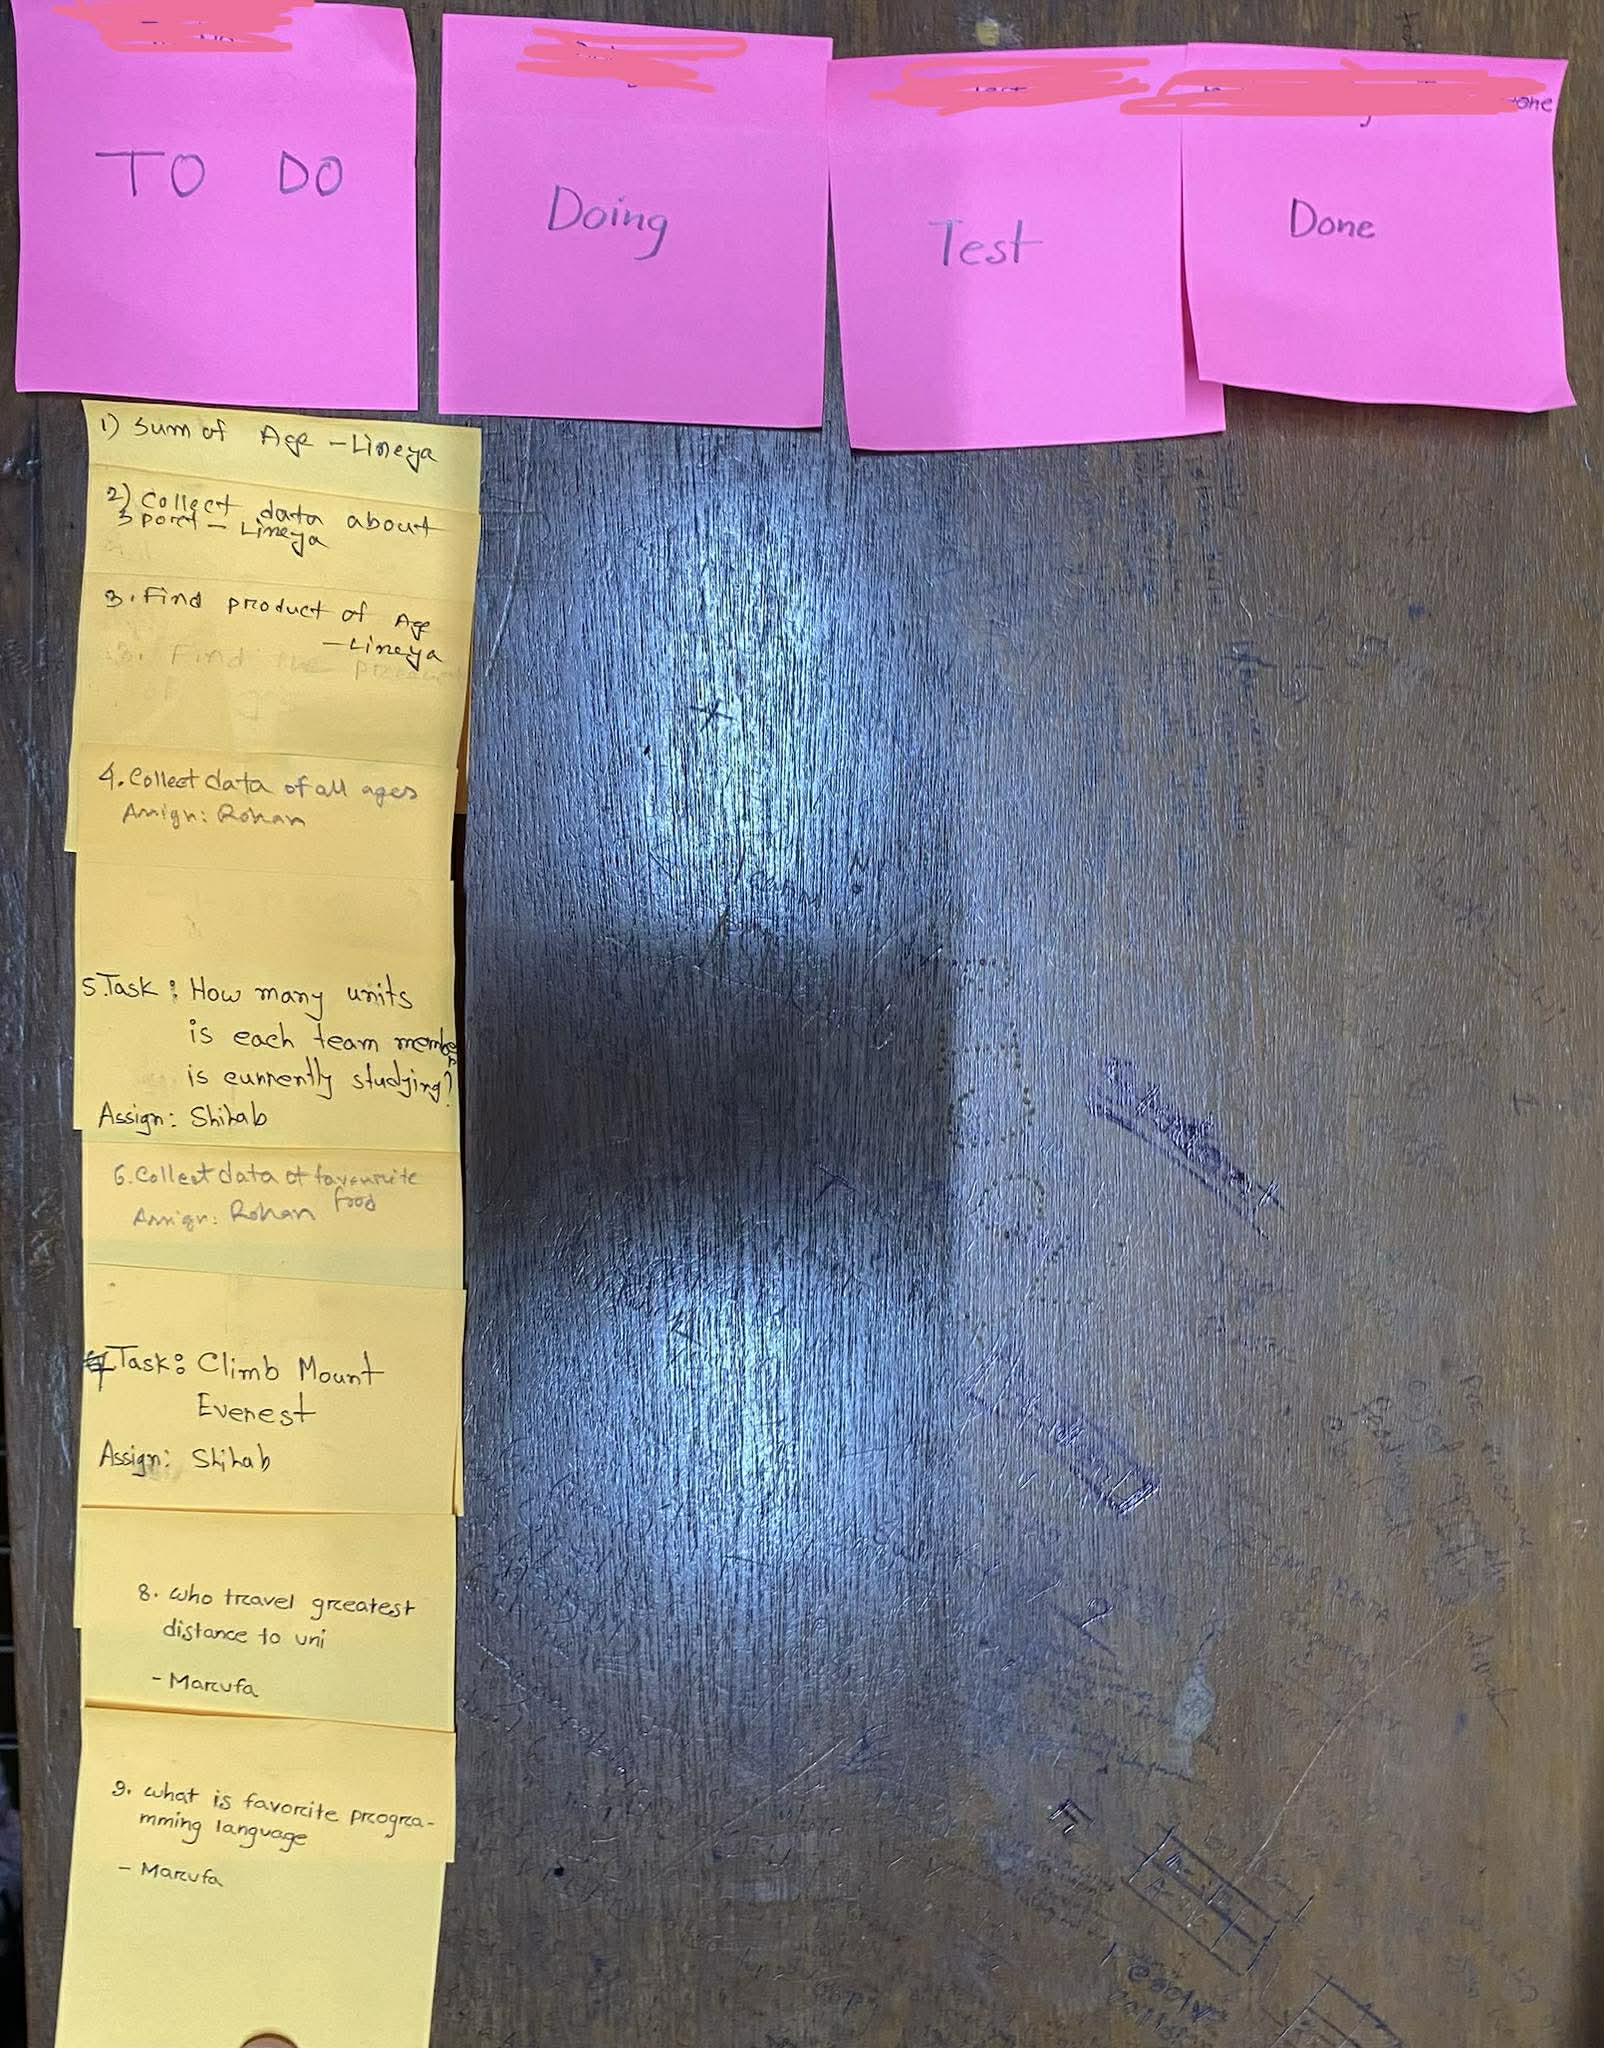
\includegraphics[width=1\textwidth]{figures/phase_1.jpg}
    \caption{phase 1}
\end{figure}
\\
\\
\\
Then 6 tasks were shifted to DOING section, basically the independent ones. The remaining tasks which were dependent stayed in the first column
\begin{figure}[H]
    \centering
    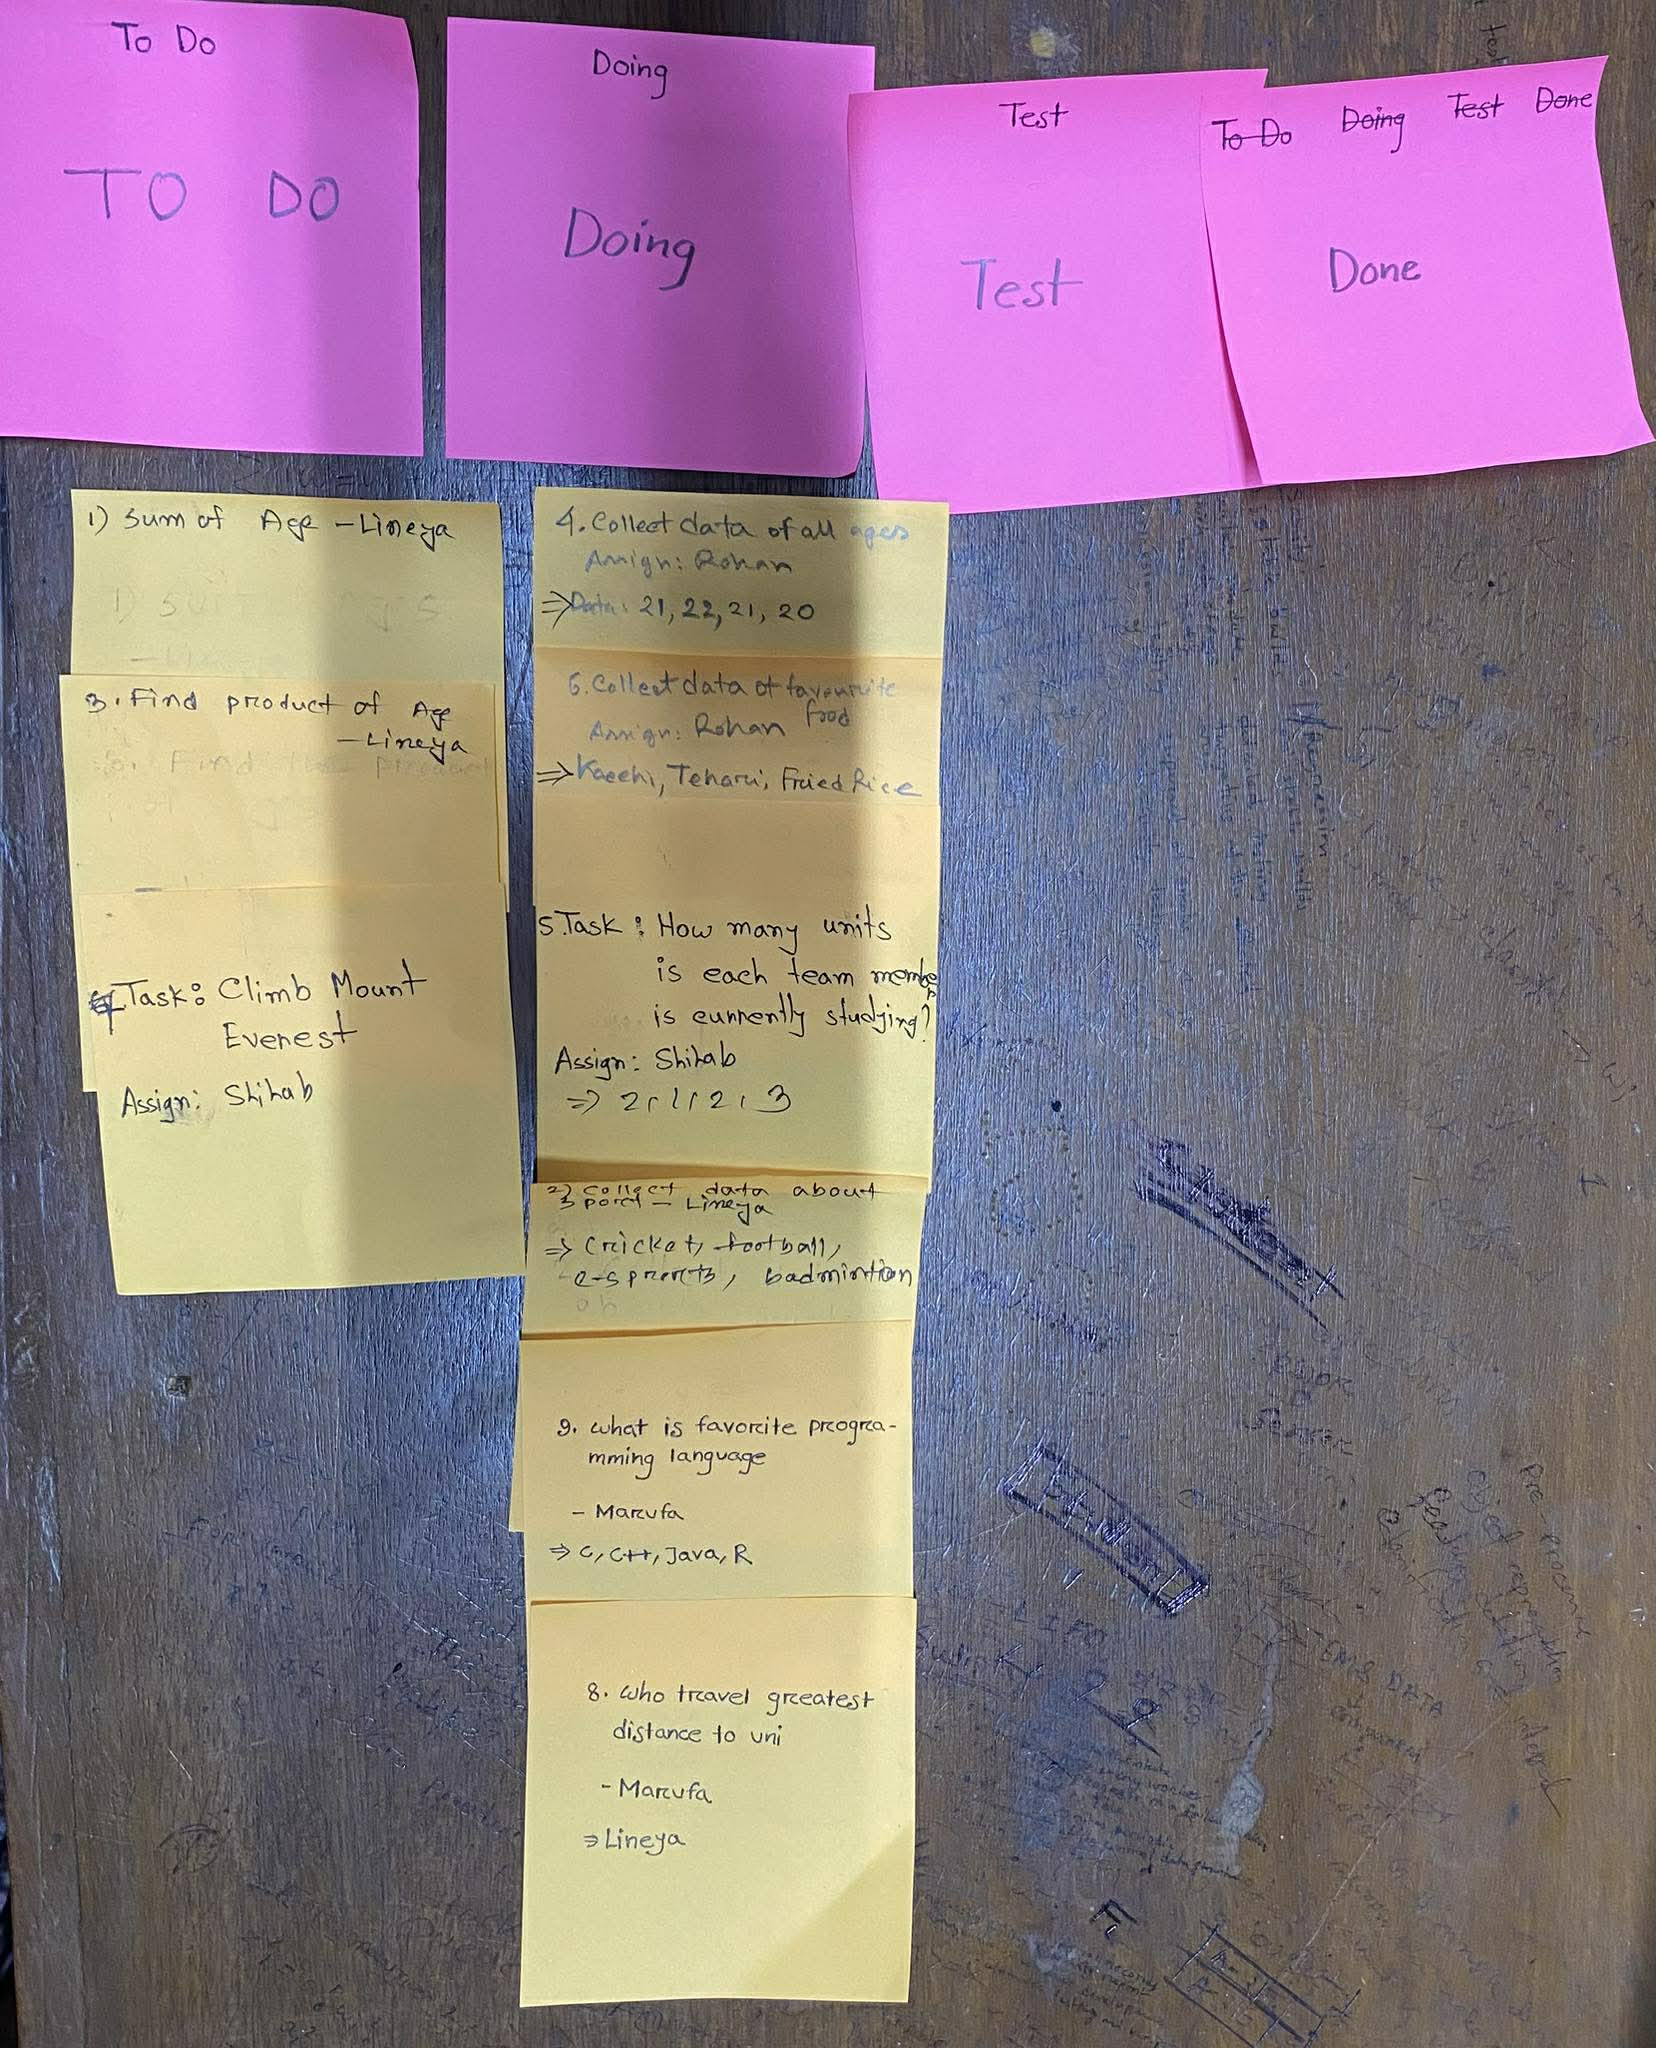
\includegraphics[width=1\textwidth]{figures/phase_2.jpg}
    \caption{phase 2}
\end{figure}
\\
\\
\\
After that 5 tasks were done without testing because most of them didn’t requite that
\begin{figure}[H]
    \centering
    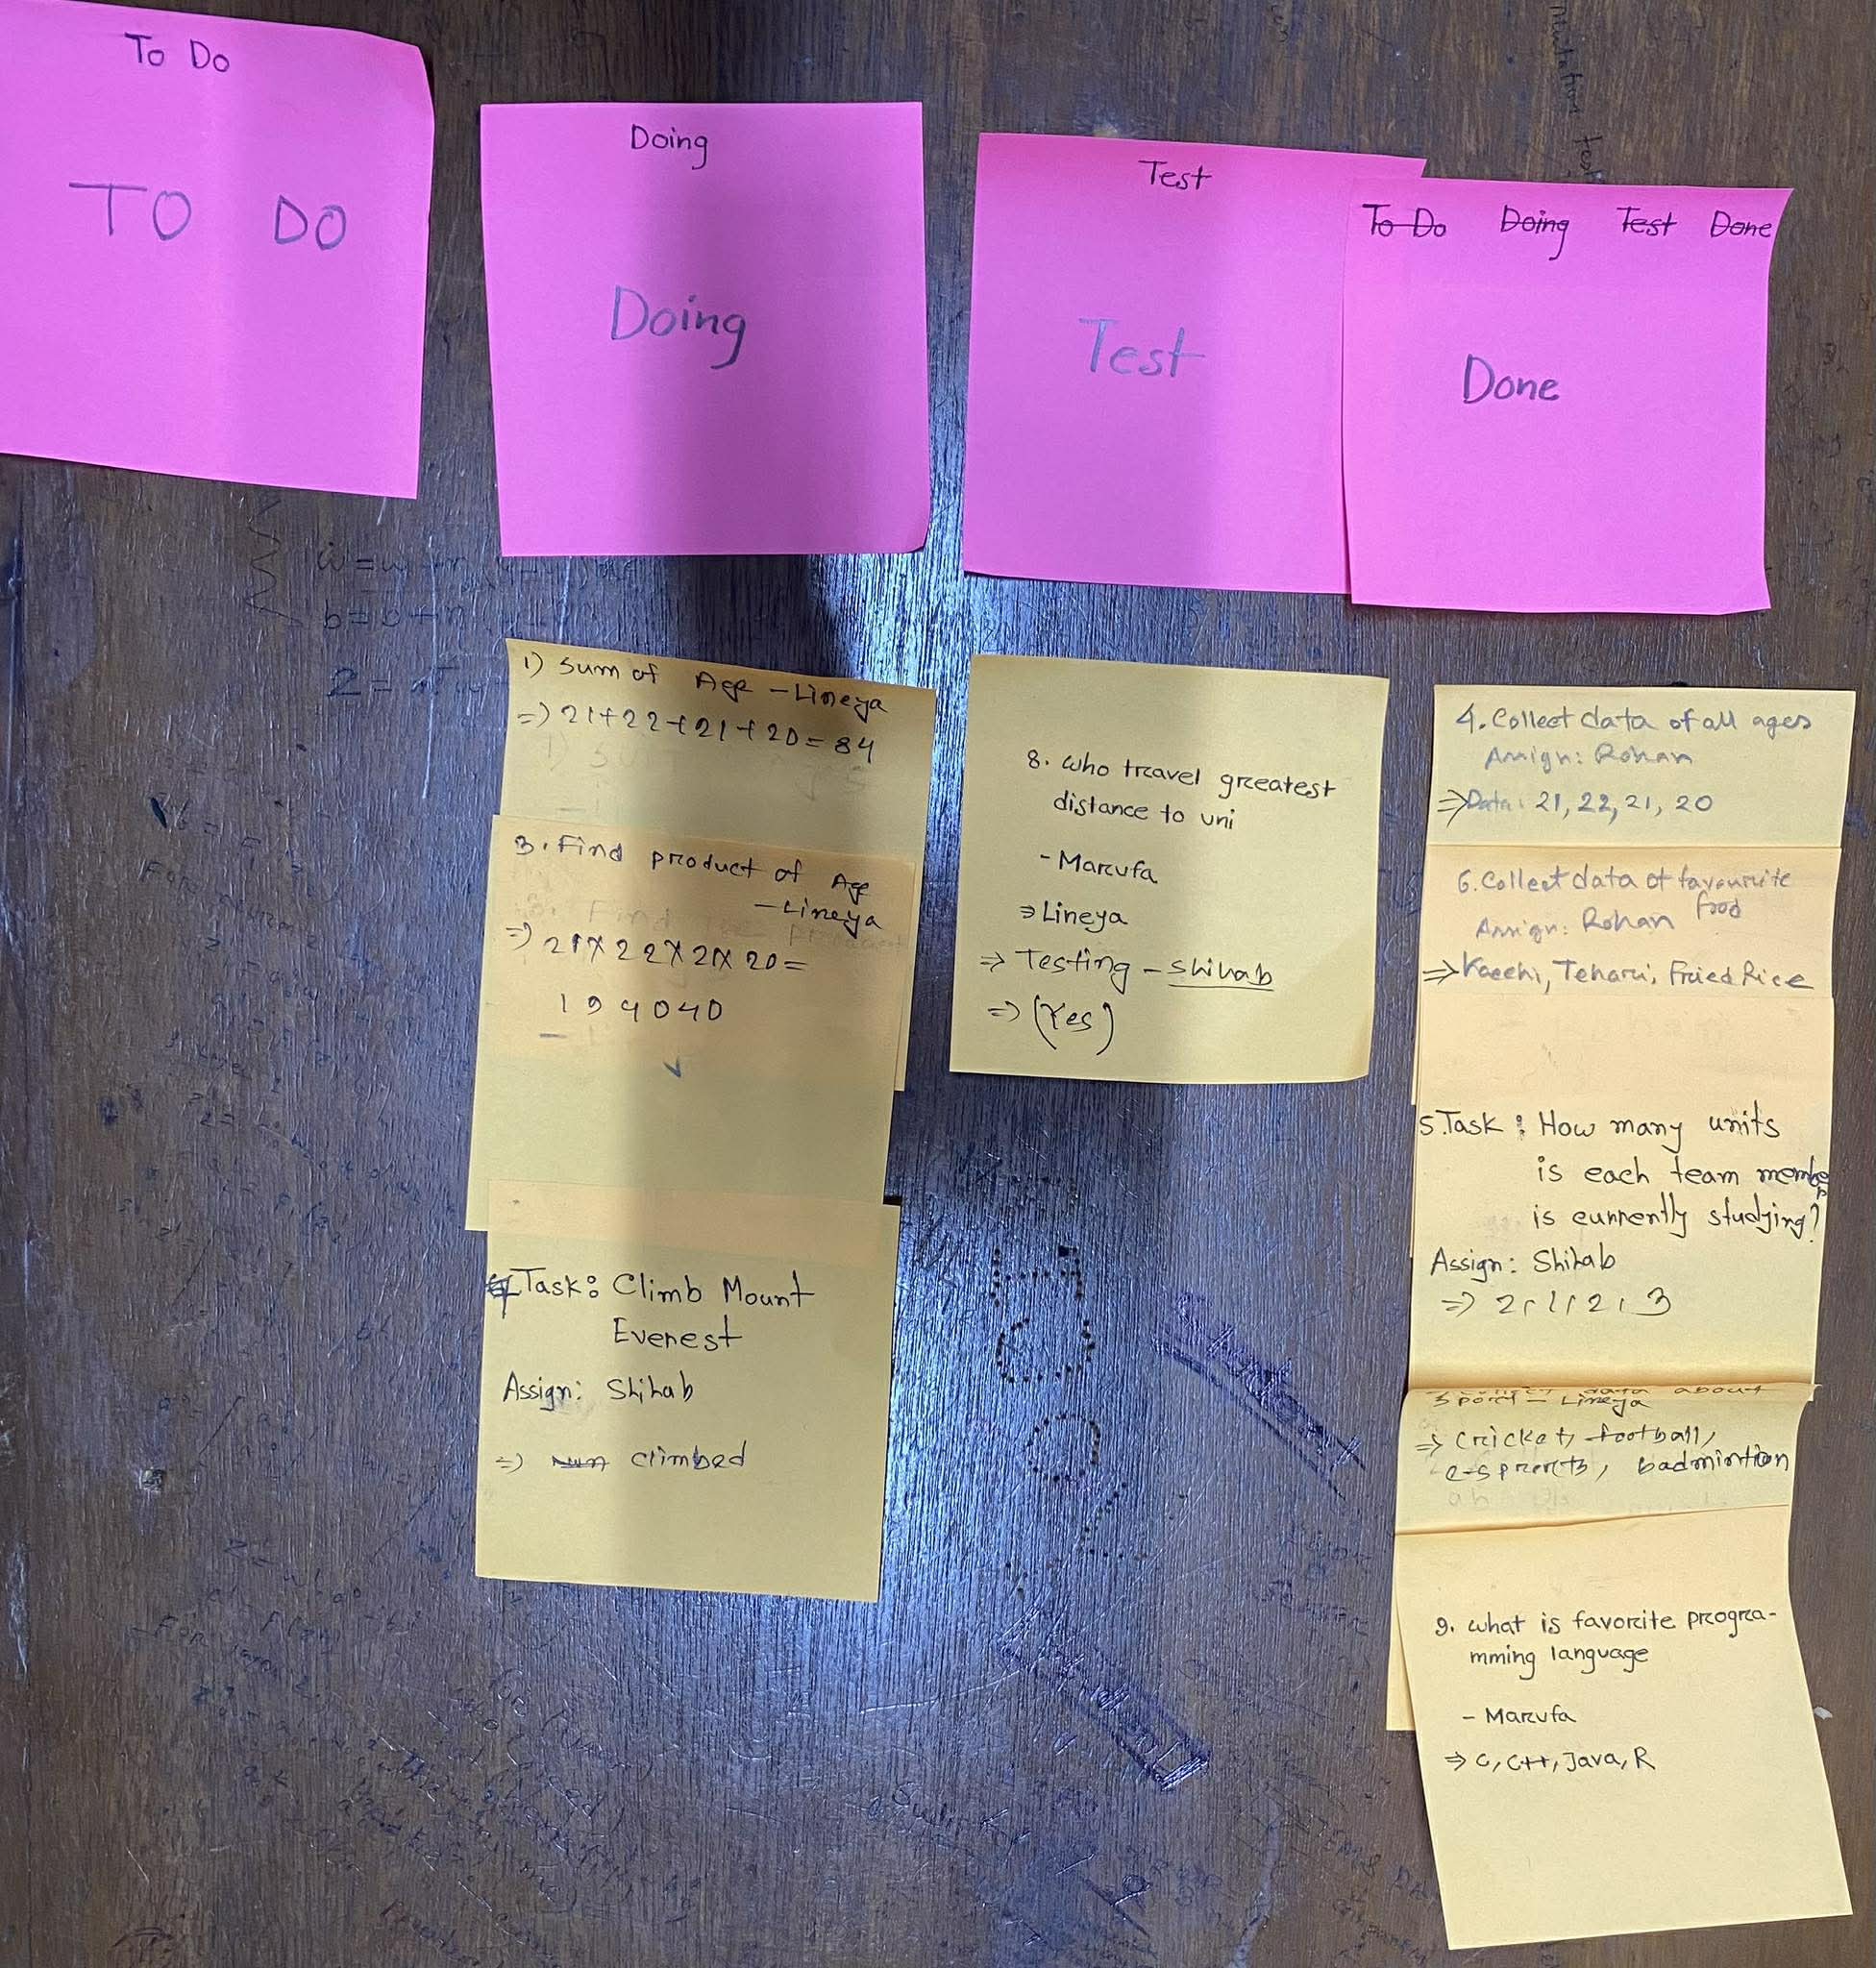
\includegraphics[width=1\textwidth]{figures/phase_3.jpg}
    \caption{phase 3}
\end{figure}
\\
\\
\\
And finally all the tasks passed the testing column. ’Climbing Mount Everest’ remained
in the doing column because it was impossible for us to climb mountain in the computer
lab. So, it got stucked in the DOING.
\begin{figure}[H]
    \centering
    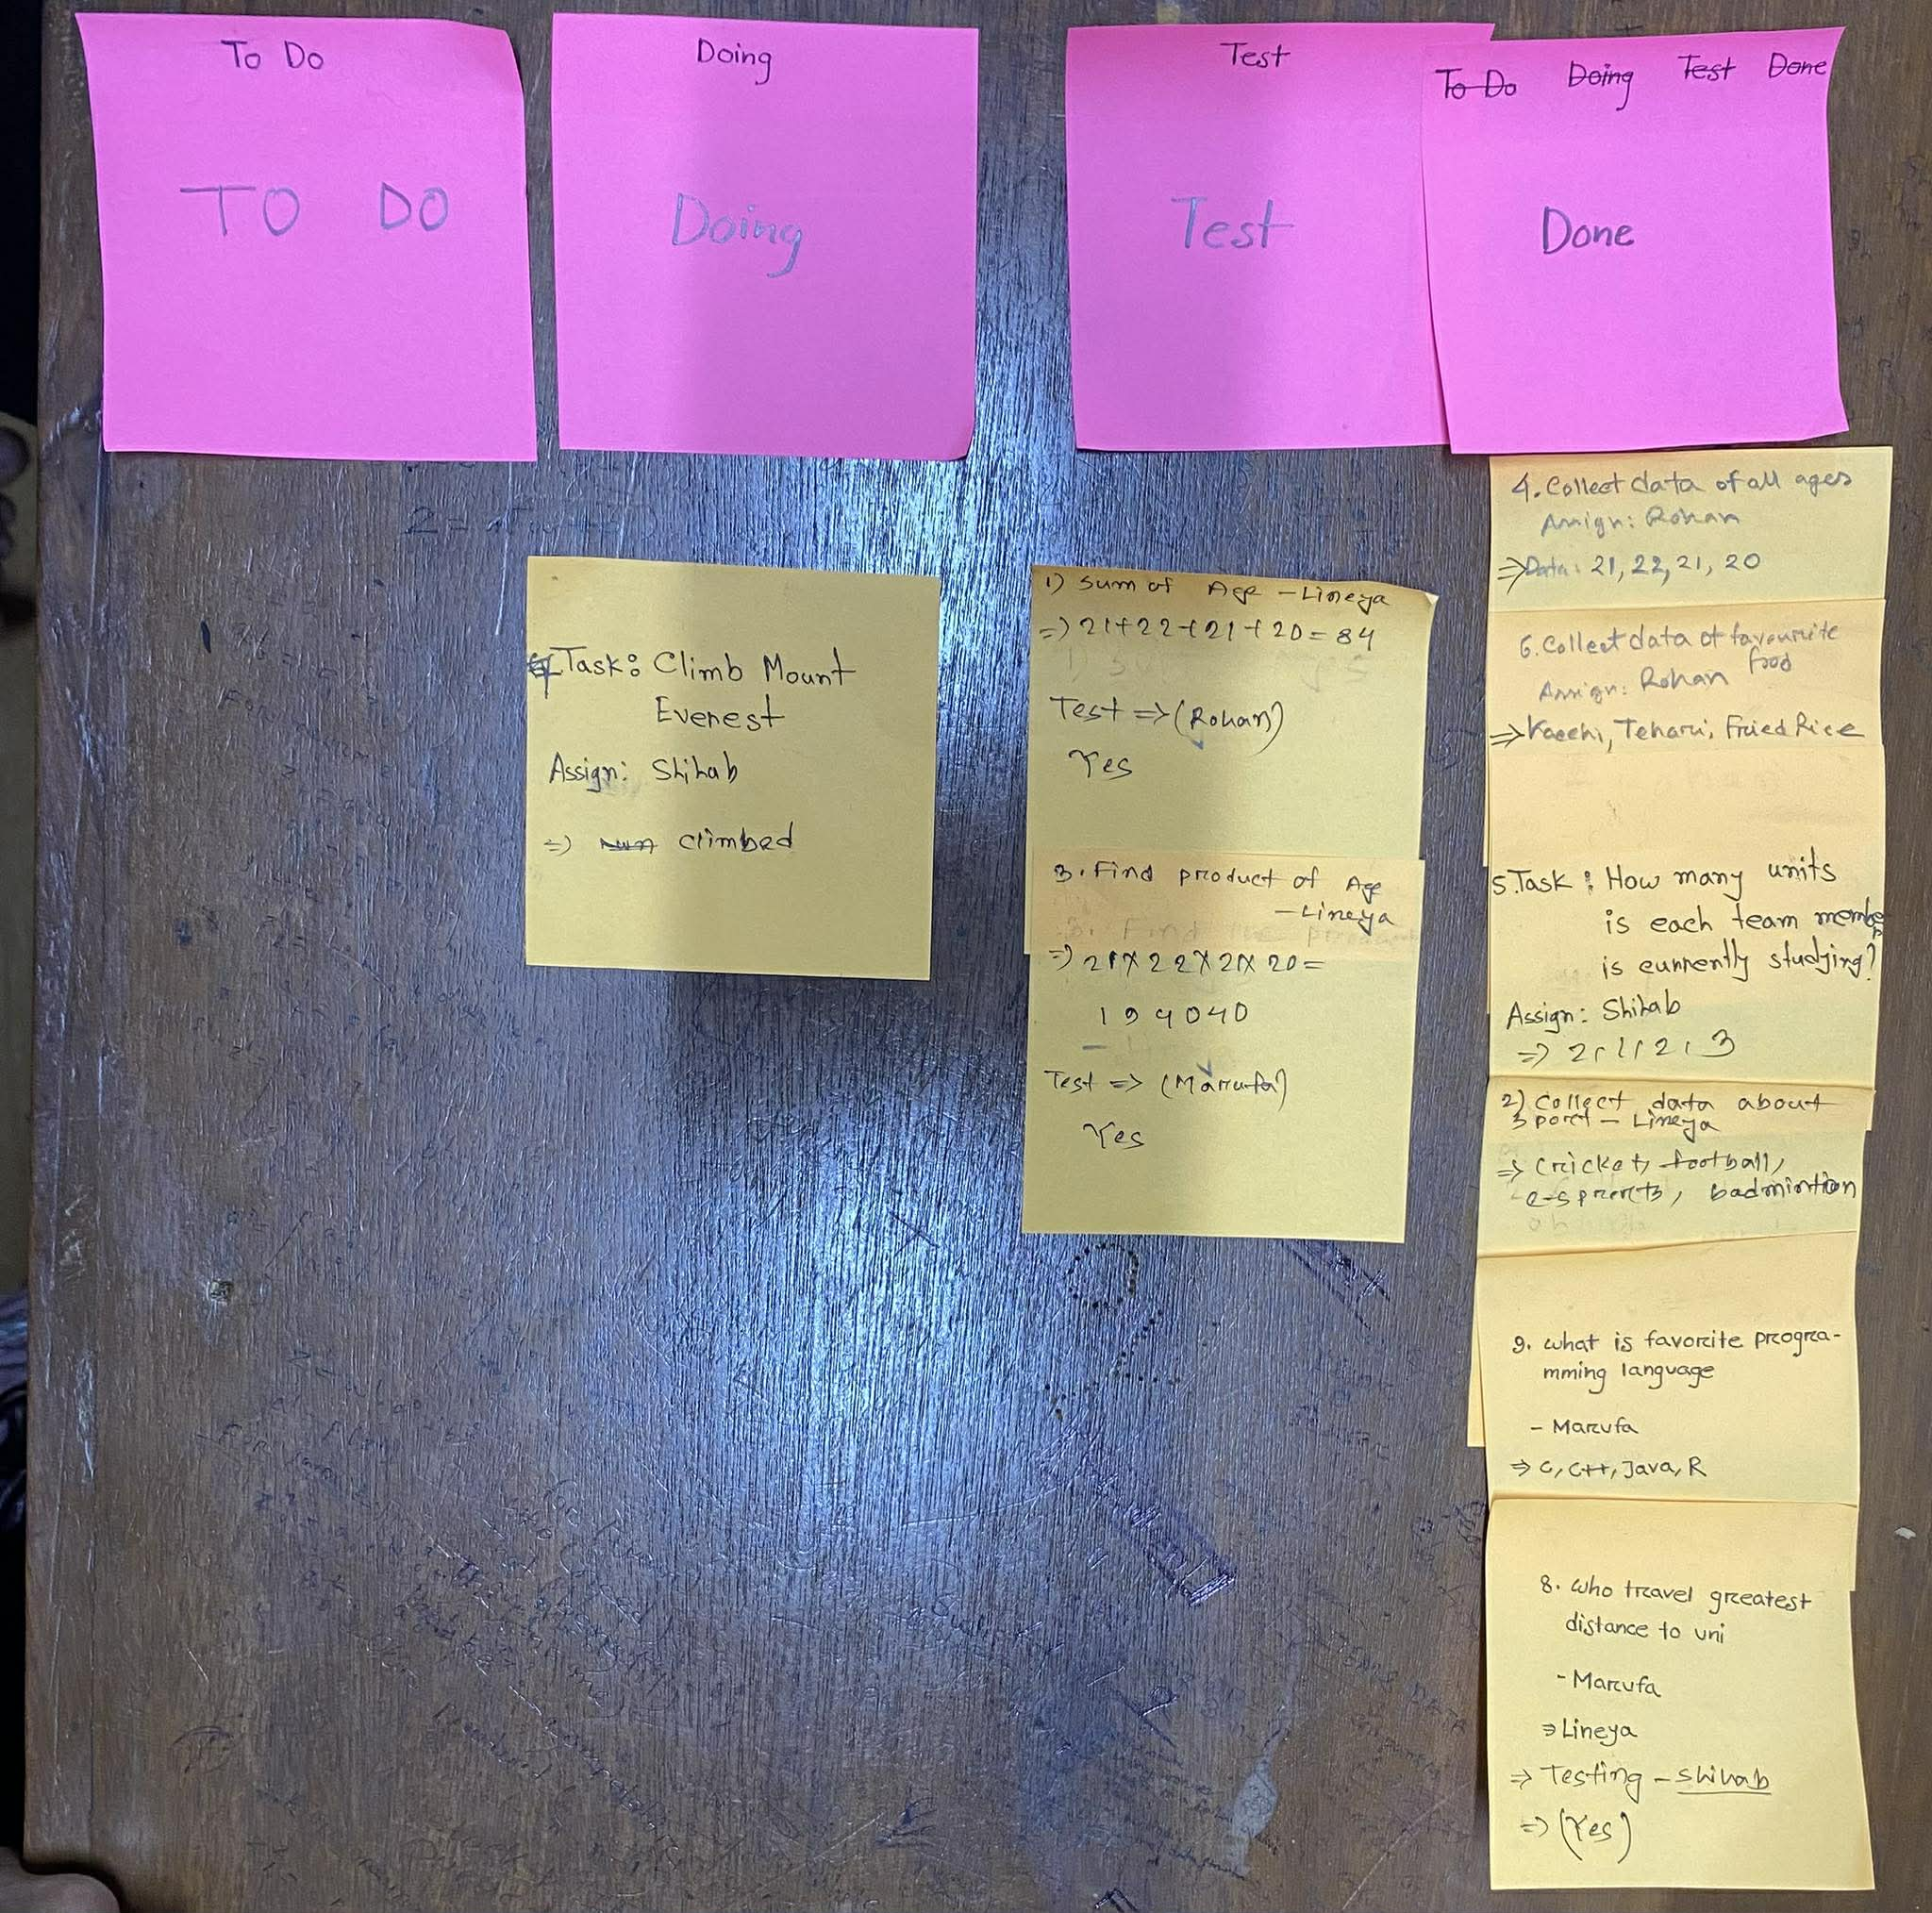
\includegraphics[width=1\textwidth]{figures/phase 4.jpg}
    \caption{phase 4}
\end{figure}
\begin{figure}[H]
    \centering
    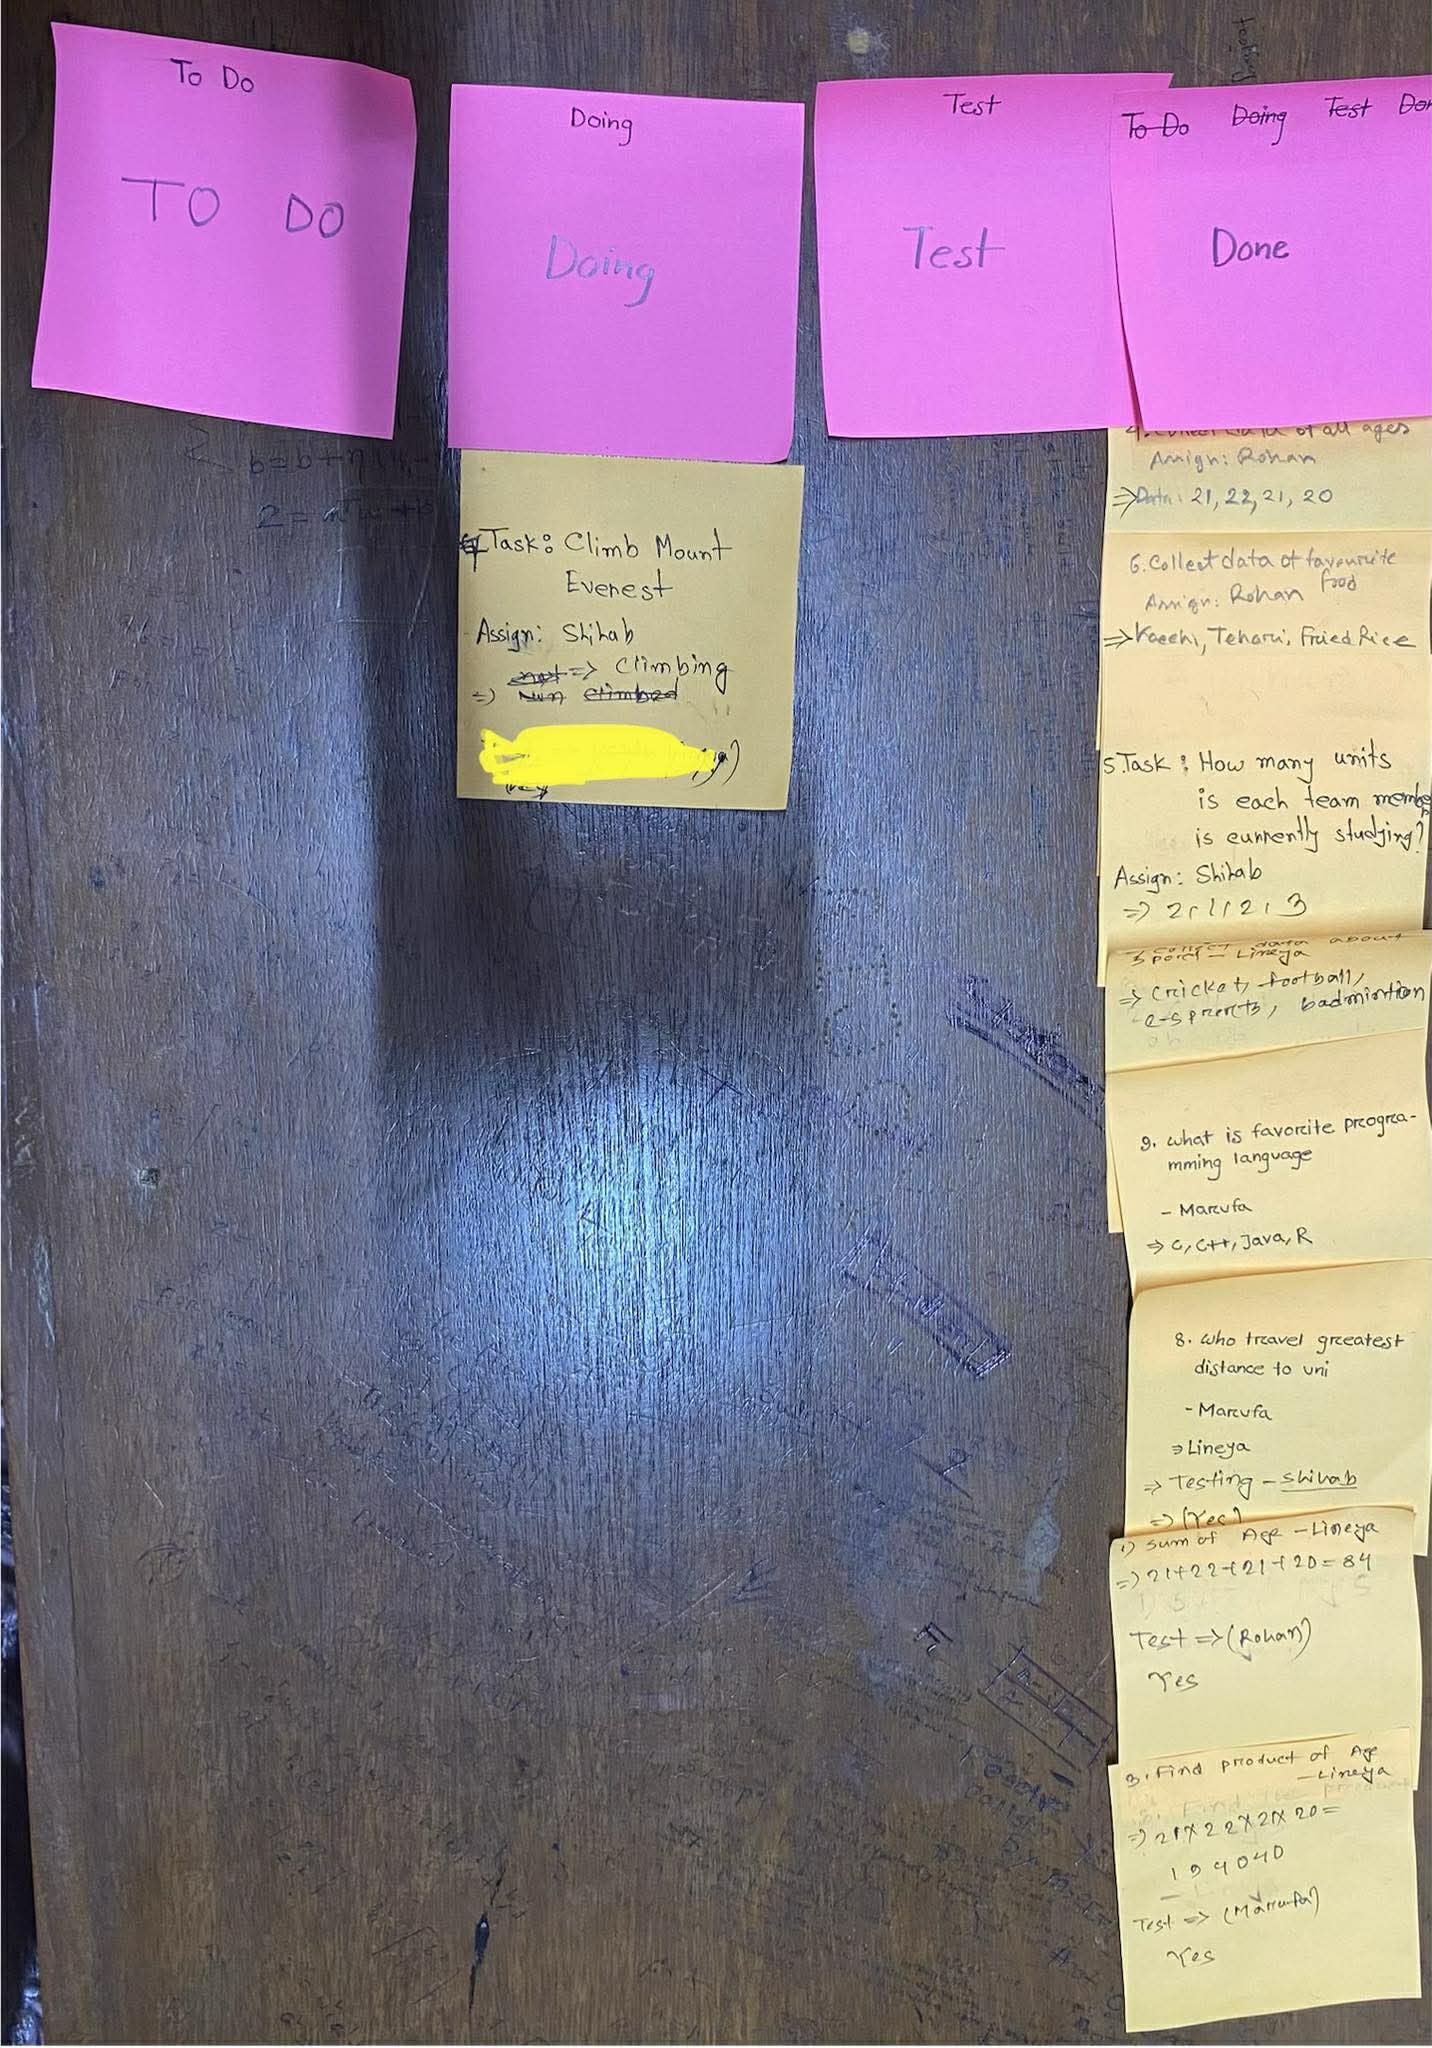
\includegraphics[width=1\textwidth]{figures/phase 5.jpg}
    \caption{phase 5}
\end{figure}
 